%!TEX root = advanced.tex

\begin{frame}{Literaturverzeichnisse mit \texorpdfstring{\BibTeX}{BibTeX}}
  \centerline{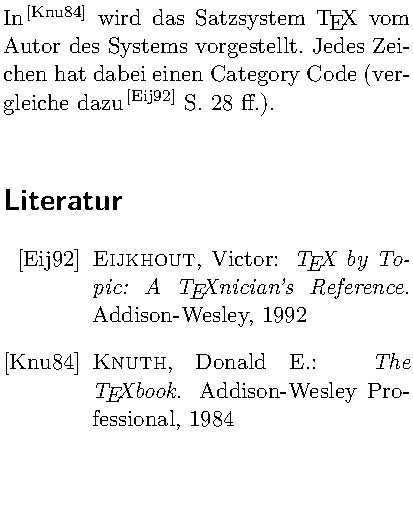
\includegraphics[width=9cm]{demo/arbeit.pdf}}
\end{frame}

\begin{frame}[fragile]{Das \LaTeX-Dokument \texttt{arbeit.tex}}
  \begin{lstlisting}[gobble=4]
    \documentclass{scrartcl}
    %...

    \begin{document}
      In \cite{Knuth} wird das Satzsystem \TeX{}
      vom Autor des Systems vorgestellt. Jedes
      Zeichen hat dabei einen Category Code
      (vergleiche dazu \cite[S.~28~ff.]{Eijkhout}).

      \bibliographystyle{alphadin}
      \bibliography{datenbank}
    \end{document}
  \end{lstlisting}
\end{frame}

\begin{frame}{Die Literaturdatenbank \texttt{datenbank.bib}}
  \lstinputlisting[language=BibTeX,moretexcs={TeX}]{demo/datenbank.bib}
\end{frame}

\begin{frame}[fragile]{Kompilieren}
  \begin{lstlisting}[language={},morekeywords={pdflatex,bibtex},gobble=4]
    pdflatex arbeit
    bibtex arbeit
    pdflatex arbeit
    pdflatex arbeit
  \end{lstlisting}

  \xxx
  \pause

  \vskip -3.1cm
  \begin{tikzpicture}
    \draw[red,very thick] (0,0) -- (2.8cm, 2.7cm);
  \end{tikzpicture}
  \vskip .5cm

  \begin{lstlisting}[language={},morekeywords={latexmk},gobble=4]
    latexmk -pdf arbeit
  \end{lstlisting}
\end{frame}

\begin{frame}{Wie funktioniert \BibTeX?}
  \begin{tikzpicture}[
      on grid,
      node distance=9mm and 23mm,
      engine/.style={
        font=\rmfamily\Large\bfseries,
        inner sep=2pt
      }
    ]

    \uncover<2->{\node[engine] (pdftex1) {\pdfTeX};}
    \uncover<1->{\node[left=40mm of pdftex1, texicon] (tex) {\icon{TEX}};}
    \uncover<1->{\node[right=40mm of pdftex1, bibicon] (bib) {\icon{BIB}};}
    \uncover<3->{\node[below left=18mm and 23mm of pdftex1, auxicon] (aux1) {\icon{AUX}};}
    \uncover<3>{\node[below right=of pdftex1, pdficon] (pdf1) {\icon{PDF}};}
    \uncover<4->{\node[below right=of pdftex1, pdficon!30] {\icon{PDF}};}
    \uncover<4->{\node[below=18mm of pdftex1, engine] (bibtex) {\BibTeX};}
    \uncover<5->{\node[below right=of bibtex, bblicon] (bbl) {\icon{BBL}};}
    \uncover<6->{\node[below=18mm of bibtex, engine] (pdftex2) {\pdfTeX};}
    \uncover<7->{\node[below left=of pdftex2, auxicon] (aux2) {\icon{AUX}};}
    \uncover<7>{\node[below right=of pdftex2, pdficon] (pdf2) {\icon{PDF}};}
    \uncover<8->{\node[below right=of pdftex2, pdficon!30] {\icon{PDF}};}
    \uncover<8->{\node[below=18mm of pdftex2, engine] (pdftex3) {\pdfTeX};}
    \uncover<9>{\node[below left=of pdftex3, auxicon] (aux3) {\icon{AUX}};}
    \uncover<10->{\node[below left=of pdftex3, auxicon!30] {\icon{AUX}};}
    \uncover<9->{\node[below right=of pdftex3, pdficon] (pdf3) {\icon{PDF}};}

    \uncover<2->{\path[very thick, ->]
      (tex) edge (pdftex1);}

    \uncover<3->{\path[very thick, ->]
      (pdftex1) edge (aux1)
                edge (pdf1);}

    \uncover<4->{\path[very thick, ->, black!30]
      (pdftex1) edge (pdf1);}

    \uncover<4->{\path[very thick, ->]
      (aux1) edge (bibtex);}

    \uncover<4->{\draw[very thick, ->]
      (bib.south) ++ (.2,0) |- (bibtex);}

    \uncover<5->{\path[very thick, ->]
      (bibtex) edge (bbl);}

    \uncover<6->{\draw[very thick, ->]
      (tex.south) ++ (.2,0) |- (pdftex2)
      (bbl.south) ++ (.2,0) |- (pdftex2);}

    \uncover<6->{\path[very thick, ->]
      (aux1) edge (pdftex2);}

    \uncover<7->{\path[very thick, ->]
      (pdftex2) edge (aux2)
                edge (pdf2);}

    \uncover<8->{\path[very thick, ->, black!30]
      (pdftex2) edge (pdf2);}

    \uncover<8->{\draw[very thick, ->]
      (tex.south) ++ (.2,0) |- (pdftex3)
      (bbl) -- (bib |- bbl) -- ++(.2,0) |- (pdftex3);}

    \uncover<8->{\path[very thick, ->]
      (aux2) edge (pdftex3);}

    \uncover<9->{\path[very thick, ->]
      (pdftex3) edge (aux3)
                edge (pdf3);}

    \uncover<10->{\path[very thick, ->, black!30]
      (pdftex3) edge (aux3);}
  \end{tikzpicture}
\end{frame}

\livecoding{\BibTeX\ in der Praxis}
